\documentclass[11pt,a4paper]{article}
\usepackage[utf8]{inputenc}
\usepackage[T1]{fontenc}
\usepackage[french]{babel}
\usepackage{lmodern}
\usepackage{geometry}
\geometry{margin=1.6cm, top=1.5cm, bottom=1.7cm}
\usepackage{graphicx}
\usepackage[table]{xcolor}
\usepackage{array,tabularx,longtable,booktabs,multirow}
\usepackage{enumitem}
\usepackage{fancyhdr}
\usepackage{titlesec}
\usepackage{hyperref}
\usepackage{caption}
\usepackage[most]{tcolorbox}
\usepackage{listings}
\usepackage{float}
\usepackage{needspace}
\usepackage{lastpage}
\usepackage{ragged2e}

\definecolor{bleuPCB}{HTML}{0B3A7A}
\definecolor{vertPCB}{HTML}{0B7F55}
\definecolor{orangePCB}{HTML}{F59E0B}
\definecolor{rougePCB}{HTML}{DC2626}
\definecolor{grisClair}{HTML}{F3F6FA}
\definecolor{grisTexte}{HTML}{2B2B2B}
\definecolor{bleuTable}{HTML}{EAF2FF}
\definecolor{vertTable}{HTML}{F2FBF7}

\hypersetup{colorlinks=true,linkcolor=bleuPCB,urlcolor=bleuPCB}
\setlength{\parindent}{0pt}
\setlength{\parskip}{4pt}
\renewcommand{\arraystretch}{1.2}
\setlist[itemize]{nosep,leftmargin=1.2em}
\setlist[enumerate]{nosep,leftmargin=1.3em}

\pagestyle{fancy}
\fancyhf{}
\lhead{EmbedLab Board -- Manuel d'utilisation}
\rhead{V1.0}
\cfoot{\thepage/\pageref{LastPage}}

\titleformat{\section}{\Large\bfseries\color{bleuPCB}}{\thesection}{0.7em}{}
\titleformat{\subsection}{\large\bfseries\color{vertPCB}}{\thesubsection}{0.7em}{}
\titleformat{\subsubsection}{\bfseries\color{grisTexte}}{\thesubsubsection}{0.7em}{}

\newcolumntype{Y}{>{\RaggedRight\arraybackslash}X}
\newcolumntype{L}[1]{>{\RaggedRight\arraybackslash}p{#1}}
\newcommand{\theadblue}[1]{\rowcolor{bleuPCB!12}\textbf{#1}}
\newcommand{\theadgreen}[1]{\rowcolor{vertPCB!10}\textbf{#1}}

\newtcolorbox{importantbox}{colback=orangePCB!10,colframe=orangePCB,title=Point critique,fonttitle=\bfseries,arc=2mm}
\newtcolorbox{warningbox}{colback=rougePCB!7,colframe=rougePCB,title=Attention,fonttitle=\bfseries,arc=2mm}
\newtcolorbox{tipbox}{colback=vertPCB!8,colframe=vertPCB,title=Conseil pratique,fonttitle=\bfseries,arc=2mm}

\lstset{basicstyle=\ttfamily\small,breaklines=true,frame=single,backgroundcolor=\color{grisClair},keywordstyle=\color{bleuPCB}\bfseries,commentstyle=\color{vertPCB},showstringspaces=false,tabsize=2,inputencoding=utf8,extendedchars=true}

\begin{document}

\begin{titlepage}
\centering
{\Huge\bfseries\color{bleuPCB} EmbedLab Board -- V1.0\\[0.25cm]}
{\Large Carte de developpement pedagogique pour systemes embarques\\[0.3cm]}
{\large Manuel d'utilisation complet\\[0.25cm]}
\vspace{0.4cm}
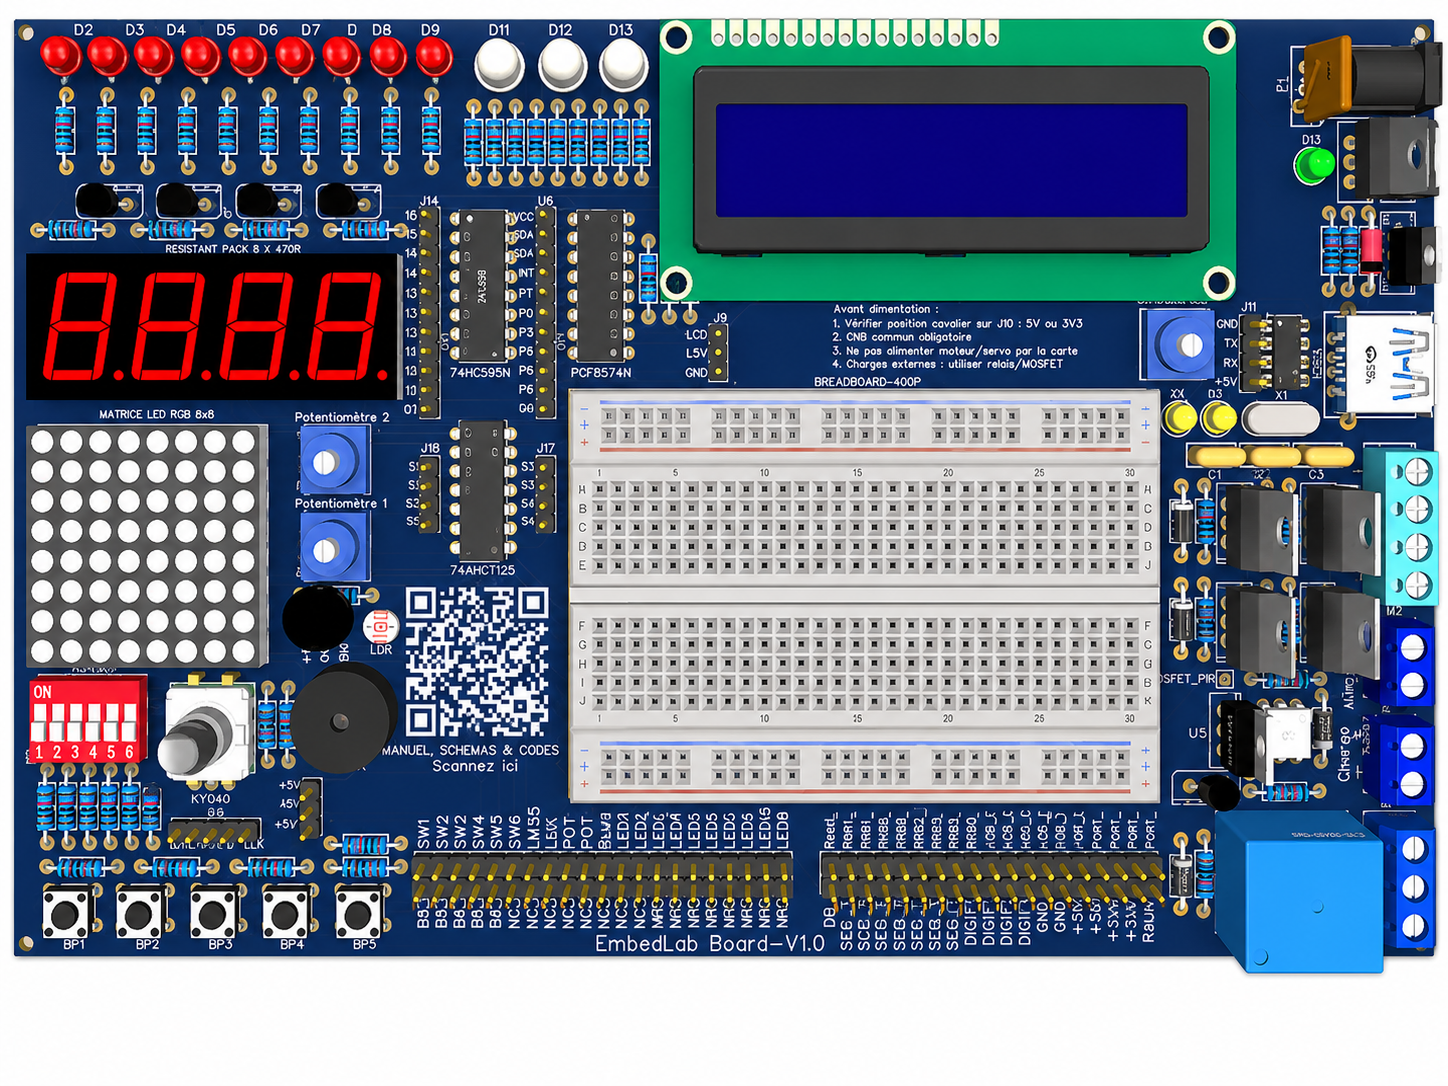
\includegraphics[width=0.98\textwidth]{../figures/cover_photo.png}
\vfill
\begin{tabular}{rl}
Projet : & Bureau d'Etudes ENA 2026 -- Sujet 5 \\
Objectif : & TP en systemes embarques, electronique et informatique industrielle \\
Version carte : & EmbedLab Board V1.0 \\
Depot GitHub : & \url{https://github.com/Scorpion160/Electronic-Development-board} \\
QR code : & manuel, schemas, fichiers EasyEDA, Gerber et codes \\
\end{tabular}
\vfill
{\small Document mis a jour avec les derniers ajustements de la carte.}
\end{titlepage}

\pagenumbering{roman}
\tableofcontents
\newpage
\pagenumbering{arabic}

\section{Presentation generale}
\textbf{EmbedLab Board} est une carte de developpement pedagogique concue pour les travaux pratiques en systemes embarques. Elle regroupe sur une meme plateforme des entrees/sorties numeriques, des capteurs analogiques, des blocs d'affichage, des interfaces de communication, une breadboard centrale et des etages de commande de puissance basse tension.

La carte n'integre pas de microcontroleur principal fixe : elle sert de \textbf{banc de TP universel}. L'etudiant y raccorde la carte de calcul de son choix : Arduino, ESP32, STM32, PIC, FPGA, Raspberry Pi Pico ou toute autre carte compatible.

\begin{importantbox}
Avant toute manipulation, verifier la position du cavalier de selection de tension logique \textbf{J10}. Placer \textbf{J10 sur 5 V} pour les microcontroleurs 5 V (Arduino Uno/Nano/MEGA classiques) et \textbf{J10 sur 3,3 V} pour ESP32, STM32, FPGA, Pico ou toute carte non tolerante 5 V.
\end{importantbox}

\subsection{Competences visees}
{\small
\begin{tabularx}{\textwidth}{@{}L{4.0cm}YY@{}}
\toprule
\rowcolor{bleuPCB!12}
\textbf{Competence} & \textbf{Modules associes} & \textbf{Ce que l'etudiant peut apprendre} \\
\midrule
GPIO numeriques & LEDs rouges et RGB, boutons BP1 a BP5, DIP-switch, relais, buzzer & Etat logique, anti-rebond, lecture/commande binaire, interruptions, validation d'etats. \\
PWM & Buzzer, MOSFET, pont en H, pilotage d'affichage ou d'actionneurs & Rapport cyclique, variation de puissance, commande d'alarme sonore ou de petits moteurs. \\
ADC & Potentiometres, LM35, LDR & Conversion analogique-numerique, calibration, mise a l'echelle, acquisition capteurs. \\
UART & CH340G, header J11, LEDs TX/RX & Communication serie avec PC, debug, journalisation de mesures. \\
I2C & PCF8574N, connectique LCD, extensions & Bus serie, adressage, pull-up, extension d'entrees/sorties. \\
SPI / logique serie & 74HC595N & Registre a decalage, sortie serie-parallele, economie de broches. \\
Compatibilite multi-cartes & J10, SN74AHCT125, headers d'acces, breadboard & Interfacage 3,3 V / 5 V, bon cablage, adaptation a la carte microcontroleur choisie. \\
Puissance basse tension & Relais, MOSFET, pont en H & Commande de charge DC, isolement, polarite, pilotage de moteur basse tension. \\
\bottomrule
\end{tabularx}}

\section{Vue d'ensemble annotee}
\begin{figure}[H]
\centering
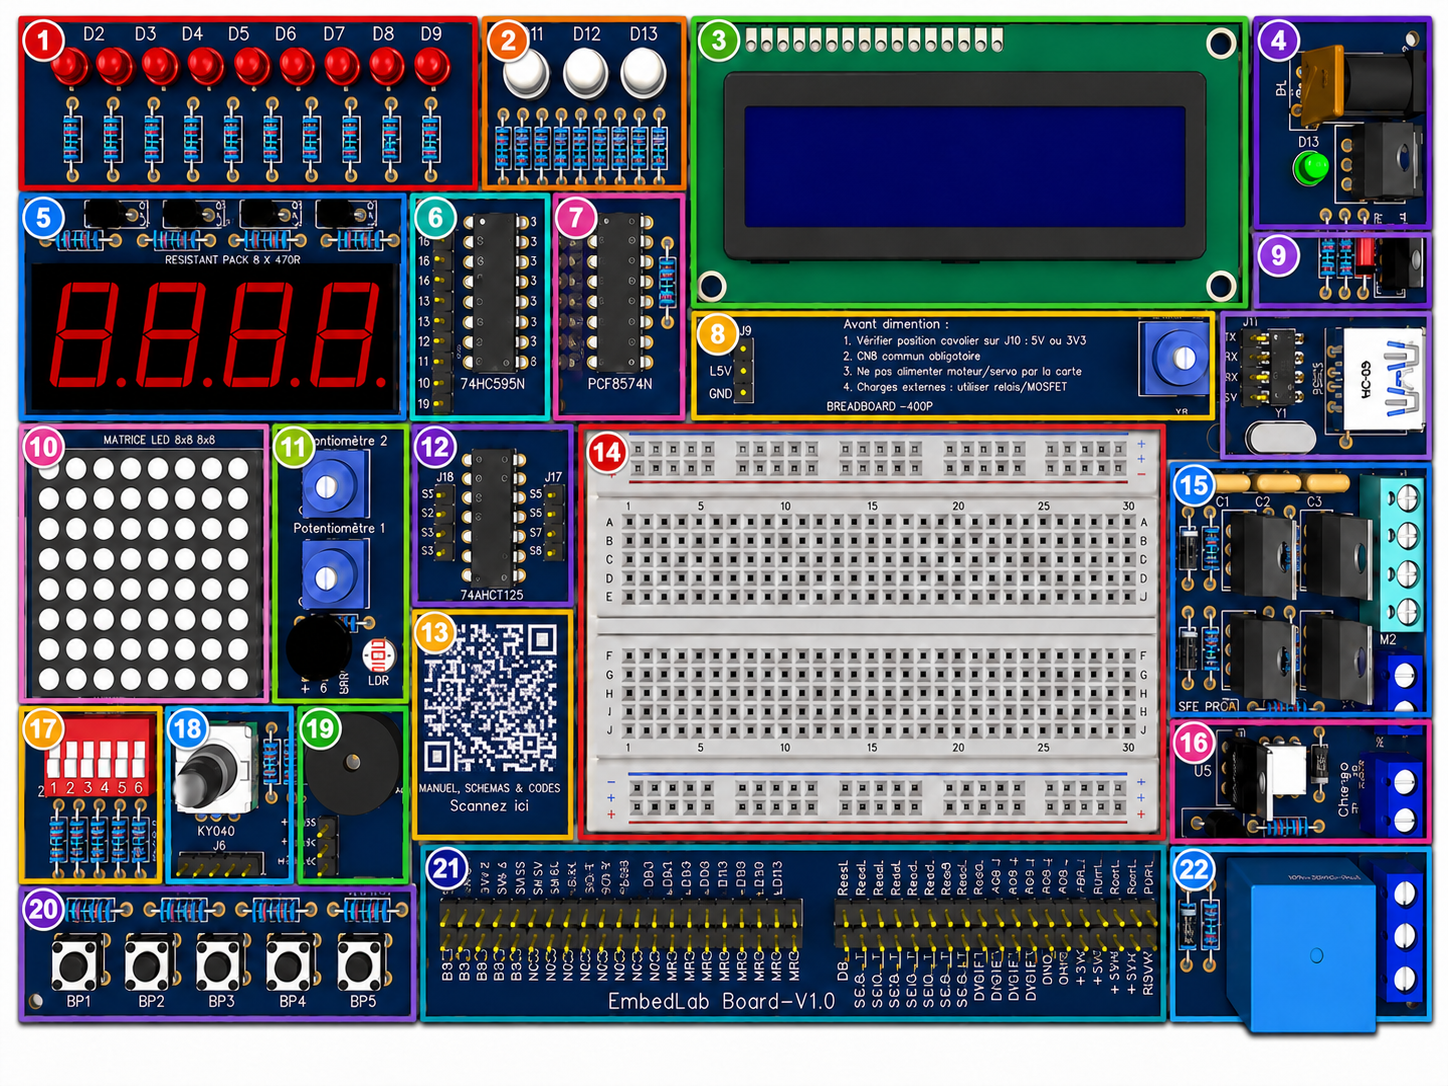
\includegraphics[width=\textwidth]{../figures/vue_3d_annotee_detaillee_v2.png}
\caption{Vue 3D annotee de l'EmbedLab Board V1.0.}
\end{figure}

\begin{center}
{\small
\begin{longtable}{@{}>{\centering\arraybackslash}p{0.9cm}>{\RaggedRight\arraybackslash}p{4.0cm}>{\RaggedRight\arraybackslash}p{11.0cm}@{}}
\toprule
\rowcolor{bleuPCB!12}
\textbf{Zone} & \textbf{Bloc / module} & \textbf{Description et usage pedagogique} \\
\midrule
\endfirsthead
\toprule
\rowcolor{bleuPCB!12}
\textbf{Zone} & \textbf{Bloc / module} & \textbf{Description et usage pedagogique} \\
\midrule
\endhead
1 & LEDs rouges D1 a D10 & Sorties numeriques simples pour TP de base : clignotement, chenillard, compteur binaire, visualisation d'etats logiques et tests de temporisation. \\
2 & LEDs RGB D11 a D13 & LEDs tricolores R/G/B pour la signalisation, la génération de couleurs et les TP de commande PWM sur plusieurs sorties. \\
3 & LCD 1602 & Affichage de messages, valeurs capteurs, menus et etats du systeme. Le LCD facilite les TP d'interface homme-machine. \\
4 & Bloc alimentation & Entree 12 V DC, fusible PTC, regulateur 5 V, regulateur 3,3 V et voyant d'alimentation. Cette zone distribue l'energie a l'ensemble de la carte. \\
5 & Afficheur 7 segments 4 digits & Affichage numerique multiplexe pour compteur, chronometre, temperature, tension ou resultat d'un ADC. \\
6 & 74HC595N & Registre a decalage serie-parallele. Ideal pour apprendre l'extension de sorties avec un nombre limite de broches microcontroleur. \\
7 & PCF8574N & Expandeur d'entrees/sorties sur bus I2C. Utile pour l'apprentissage du bus I2C et des GPIO additionnelles. \\
8 & Rappel de mise sous tension / J9 & Zone de rappel des consignes critiques : verifier J10, utiliser un GND commun, ne pas alimenter moteur/servo par la logique et reserver les charges externes au relais, au MOSFET ou au pont en H. \\
9 & Interface USB-serie CH340G & Liaison UART avec le PC, connecteur USB, quartz et LEDs TX/RX. Cette zone sert au debug serie et aux TP de communication. \\
10 & Matrice LED 8x8 & Affichage matriciel pour caracteres, balayage ligne/colonne, animations et petits jeux ou pictogrammes. \\
11 & Entrees analogiques et capteurs & Deux potentiometres, LM35 et LDR. Cette zone sert aux TP de mesure, de conversion ADC et de traitement de donnees capteurs. \\
12 & SN74AHCT125 et J17/J18 & Adaptation de niveaux logiques, particulierement utile pour interfacer des signaux 3,3 V avec des entrees ou circuits 5 V. \\
13 & QR code du projet & Acces direct au depot GitHub contenant le manuel, la fiche rapide, les schemas, les Gerber, les fichiers EasyEDA et les exemples de code. \\
14 & Breadboard 400 points & Zone de prototypage sans soudure. Permet d'ajouter des montages de TP, des microcontroleurs, des capteurs externes ou des essais rapides. \\
15 & Pont en H & Etage de commande pour petit moteur DC basse tension. Permet l'etude du sens de rotation et de la commande moteur. \\
16 & MOSFET / charge DC externe & Etage de commande d'une charge DC via MOSFET. Convient a une lampe, une charge resistive ou un petit actionneur DC. \\
17 & DIP-switch 6 positions & Configuration manuelle de modes, adresses, options de TP ou conditions initiales sans modifier le code. \\
18 & Encodeur rotatif KY040 & Reglage de consigne, navigation dans un menu LCD, mesure d'increment et apprentissage des entrees quadrature. \\
19 & Buzzer & Signal sonore, bips de validation, alarme et generation de tonalites simples. \\
20 & Boutons BP1 a BP5 & Entrees utilisateur pour validation, changement de mode, interruption et TP d'anti-rebond. \\
21 & Headers d'acces aux signaux & Broches d'interconnexion vers le microcontroleur externe ou vers la breadboard. C'est la zone cle de cablage pour tous les TP. \\
22 & Relais SRD 5 V & Commande d'une charge externe basse tension avec isolement entre commande et puissance. \\
\bottomrule
\end{longtable}}
\end{center}

\begin{tipbox}
Les zones repérées sur la figure permettent d’identifier rapidement les différents blocs de la carte : alimentation, affichage, entrées, sorties, capteurs, interfaces logiques, communication et commande de puissance. Cette organisation facilite la prise en main de la carte et le câblage des manipulations.
\end{tipbox}

\section{Alimentation et securite}
\subsection{Architecture generale}
La carte est alimentee par une entree \textbf{12 V DC}. Cette entree passe par un fusible PTC de protection puis alimente les regulateurs linaires 5 V et 3,3 V. Le 5 V sert a la logique TTL, au LCD, au CH340G et a plusieurs modules internes. Le 3,3 V est destine aux signaux et microcontroleurs non tolerants 5 V.

\begin{warningbox}
Les regulateurs \textbf{LM7805} et \textbf{LM1117T-3.3} sont lineaires. Ils dissipent de la chaleur. Il ne faut donc \textbf{jamais} alimenter moteur, servo ou charge de puissance directement depuis le 5 V logique de la carte. Utiliser une alimentation externe pour la puissance et commuter cette charge via le relais, le MOSFET ou le pont en H.
\end{warningbox}

{\small
\begin{tabularx}{\textwidth}{@{}L{4.0cm}YY@{}}
\toprule
\rowcolor{bleuPCB!12}
\textbf{Element} & \textbf{Role} & \textbf{Consigne pratique} \\
\midrule
Entree 12 V DC & Alimentation principale de la carte & Utiliser une alimentation stable, polarite respectee et courant adapte au TP. \\
Fusible PTC & Protection contre les surintensites & En cas de declenchement, couper l'alimentation, corriger le defaut puis attendre le refroidissement. \\
LM7805 & Generation du 5 V logique & A reserver a la logique et aux petits modules, pas aux charges gourmandes. \\
LM1117T-3.3 & Generation du 3,3 V logique & A utiliser pour capteurs, signaux et cartes 3,3 V. \\
J10 & Selection de la reference logique & A verifier avant toute lecture analogique ou raccordement GPIO. \\
GND commun & Reference commune avec la carte externe & Obligatoire pour toutes les mesures et commandes non isolees. \\
\bottomrule
\end{tabularx}}

\subsection{Cavalier J10 : regle a retenir}
\begin{importantbox}
\textbf{J10 = 5 V} pour Arduino Uno, Nano, Mega et autres cartes logiques 5 V. \\
\textbf{J10 = 3,3 V} pour ESP32, STM32, FPGA, Pico et toutes les cartes non tolerantes 5 V. \\
Toujours verifier J10 avant d'utiliser \textbf{POT1, POT2, LM35 ou LDR}. Une mauvaise position du cavalier peut envoyer un niveau trop eleve vers une entree analogique sensible.
\end{importantbox}

\section{Connecteurs et cablage}
\subsection{Headers principaux}
{\small
\begin{tabularx}{\textwidth}{@{}L{2.2cm}L{4.5cm}Y@{}}
\toprule
\rowcolor{bleuPCB!12}
\textbf{Connecteur} & \textbf{Broches / signaux} & \textbf{Utilisation} \\
\midrule
J1 & LED1 a LED10 & Commande des LEDs rouges. \\
J2 & D11 a D13 & Commande des trois LEDs RGB. \\
J3 & Buzzer & Commande du buzzer. \\
J4 & BP1 a BP5 & Lecture des boutons poussoirs. \\
J5 & MOSFET & Commande de l'etage MOSFET pour charge DC. \\
J6 & K1, K2, K3, K4 & Commande des interrupteurs du pont en H. \\
J7 / J8 & Lignes et colonnes matrice 8x8 & Pilotage de la matrice LED. \\
J9 & LM35, LDR, POT1, POT2 & Lecture des entrees analogiques. \\
J10 & 5 V / 3,3 V & Selection de la tension logique des entrees et capteurs. \\
J11 & GND, TX, RX, +5V & Interface serie issue du CH340G. \\
J12 & Encodeur KY040 & Signaux CLK, DT, SW, plus alimentation de l'encodeur. \\
J13 & Q0 a Q7 & Sorties paralleles du 74HC595N. \\
J14 & DS, ST et SH & Connecteur de commande du 74HC595N. \\
J15 & P0 a P7 & Connecteur des 8 entrees/sorties programmables du PCF8574N. \\
J16 & SDA, SCL et INT & Connecteur de communication du PCF8574N. \\
J17 / J18 & E1-S1, E2-S2, E3-S3, E4-S4 & Conversion de niveau via SN74AHCT125. \\
J19 & Alimentation LCD & Pemet d'eteindre le LCD lorsqu'on ne l'utilise pas. \\
H1 & Segments, digits et DP & Pilotage de l'afficheur 7 segments 4 digits. \\
P6 & Rs, E, D4, D5, D6 et D7 & Pilotage de l'ecran LCD. \\
P8 & GND, 5V, 3V3 & Sorties disponibles pour alimenter le breadboard. \\
10K1 & Relais & Commande la charge AC/DC apartir du relais. \\
\bottomrule
\end{tabularx}}

\begin{figure}[H]
\centering
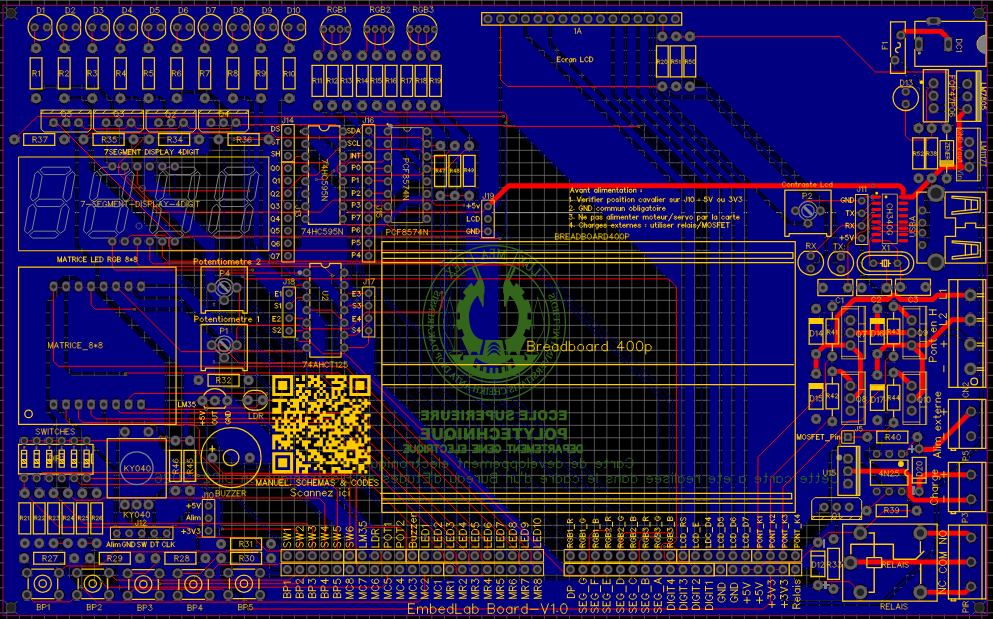
\includegraphics[width=\textwidth]{../figures/routage.png}
\caption{Extrait du routage montrant les connecteurs d'acces aux signaux.}
\end{figure}

\subsection{Connecteurs de puissance et broches a reperer}
{\small
\begin{tabularx}{\textwidth}{@{}L{2.8cm}L{4.4cm}Y@{}}
\toprule
\rowcolor{bleuPCB!12}
\textbf{Bloc} & \textbf{Broches a identifier} & \textbf{Precautions} \\
\midrule
Relais & COM, NO, NC & Utiliser de preference une charge DC basse tension en TP. Bien identifier la borne commune et l'etat au repos. \\
Pont en H & Alim moteur, M1, M2, commandes logiques & Verifier l'alimentation moteur, ne jamais court-circuiter une branche haut/bas et rester sur un petit moteur DC basse tension. \\
MOSFET & Charge + / charge -, commande, GND & La charge externe peut etre alimentee separement. Relier les masses si le montage n'est pas isole. \\
Alimentation externe & 12 V entree, GND, eventuels borniers de puissance & Respecter polarite et tension. Ne pas inverser le cablage. \\
USB-serie & GND, TX, RX, +5 V & Croiser TX vers RX du microcontroleur, conserver un GND commun. \\
\bottomrule
\end{tabularx}}

\section{Modules d'entree}
\subsection{Boutons BP1 a BP5}
Les boutons poussoirs permettent de generer des entrees logiques. Ils peuvent servir a valider un choix, changer de mode, lancer une mesure ou declencher une interruption.

\begin{lstlisting}[language=C,caption={Lecture simple d'un bouton avec Arduino}]
const int BP1 = 2;
const int LED = 13;

void setup() {
  pinMode(BP1, INPUT_PULLUP);  // adapter selon le cablage reel
  pinMode(LED, OUTPUT);
}

void loop() {
  bool appui = (digitalRead(BP1) == LOW);
  digitalWrite(LED, appui ? HIGH : LOW);
}
\end{lstlisting}

\subsection{DIP-switch 6 positions}
Le DIP-switch permet de configurer rapidement un mode de fonctionnement sans reprogrammer la carte : choix de TP, activation d'une option, selection d'adresse ou configuration d'un scenario.

\subsection{Encodeur KY040}
L'encodeur rotatif KY040 permet de detecter des increments de rotation et parfois un appui. Il est pratique pour regler une consigne, naviguer dans un menu ou tester la lecture d'un codeur.

\subsection{Entrees analogiques : POT1, POT2, LM35 et LDR}
Les deux potentiometres fournissent une tension variable. Le LM35 fournit une tension proportionnelle a la temperature, tandis que la LDR varie avec l'eclairement. Ces signaux sont accessibles au microcontroleur via les headers inferieurs.

\begin{warningbox}
Avant de brancher une entree analogique vers un ESP32, un STM32 ou un FPGA, verifier que \textbf{J10 est sur 3,3 V}. Ne jamais supposer que le signal est deja limite a 3,3 V.
\end{warningbox}

\begin{lstlisting}[language=C,caption={Lecture d'un potentiometre}]
const int POT = A0;

void setup() {
  Serial.begin(9600);
}

void loop() {
  int adc = analogRead(POT);
  Serial.println(adc);
  delay(200);
}
\end{lstlisting}

\section{Modules de sortie}
\subsection{LEDs simples}
La carte dispose d'un groupe de LEDs rouges et d'un groupe de LEDs RGB. Ces sorties permettent les TP de base sur GPIO : clignotement, chenillard, visualisation d'etats et tests de sequence, commande PWM et génération de couleurs.

\subsection{Buzzer}
Le buzzer permet de produire une alarme ou des bips de validation. Il peut etre pilote en tout ou rien ou via un signal periodique pour generer differentes tonalites.

\section{Affichage}
\subsection{LCD 1602}
Le LCD 16x2 sert a afficher les mesures, les messages d'etat ou un menu simple. Le contraste doit etre ajuste si necessaire, et l'alimentation du LCD doit rester coherente avec le TP.

\subsection{Afficheur 7 segments 4 digits}
L'afficheur 7 segments permet de travailler le multiplexage, la decomposition d'un nombre en digits et l'affichage rapide de valeurs numeriques.

\subsection{Matrice LED 8x8}
La matrice LED 8x8 permet l'affichage matriciel, les animations simples, les caracteres et l'apprentissage du balayage ligne/colonne.

\section{Circuits d'extension logique}
\subsection{74HC595N}
Le 74HC595N est un registre a decalage. Il recoit les bits en serie et les restitue sur des sorties paralleles. Il est tres utile pour economiser les broches GPIO.

\subsection{PCF8574N}
Le PCF8574N est un expandeur d'entrees/sorties I2C. Il permet d'augmenter le nombre de GPIO a partir des lignes SDA et SCL.

\subsection{SN74AHCT125}
Le SN74AHCT125 aide a l'adaptation de niveaux logiques, en particulier quand un signal issu d'une carte 3,3 V doit piloter proprement un circuit attendu en 5 V.

\section{Communication USB-serie}
La carte integre un \textbf{CH340G} pour la communication UART avec le PC. Le header J11 expose typiquement \textbf{GND, TX, RX et +5 V}. Les LEDs TX/RX donnent un retour visuel de l'activite serie.

\begin{lstlisting}[language=C,caption={Test de communication serie}]
void setup() {
  Serial.begin(9600);
}

void loop() {
  Serial.println("EmbedLab Board OK");
  delay(1000);
}
\end{lstlisting}

\section{Commande de puissance basse tension}
\subsection{Relais SRD-DC5V-SL-C}
Le relais commute une charge externe en separant la commande logique du circuit de puissance. Pour les TP, il est recommande de rester en basse tension continue.

\begin{warningbox}
Pour un usage etudiant, ne pas utiliser le relais avec le secteur 230 V. Utiliser une charge DC basse tension, avec un courant limite et sous surveillance.
\end{warningbox}

\subsection{MOSFET IRFZ44N}
Le MOSFET commande une charge DC externe en tout ou rien ou en PWM. Si la charge consomme beaucoup, utiliser une alimentation separee pour la puissance et relier les masses quand le montage n'est pas isole.

\subsection{Pont en H}
Le pont en H permet de faire tourner un petit moteur DC dans les deux sens. Les quatre commandes doivent etre pilotees correctement pour eviter tout court-circuit interne entre l'alimentation et la masse.

\begin{warningbox}
Ne jamais activer simultanement le transistor haut et le transistor bas d'une meme branche. Pour les essais, choisir un petit moteur DC basse tension et limiter le courant.
\end{warningbox}

\section{Procedure de prise en main rapide}
\begin{enumerate}
\item Inspecter visuellement la carte et verifier l'absence de court-circuit ou de composant mal oriente.
\item Verifier \textbf{J10} selon le microcontroleur utilise.
\item Connecter le \textbf{GND commun} entre la carte et le microcontroleur externe.
\item Alimenter la carte et verifier les voyants d'alimentation.
\item Choisir un module simple a tester : LED, bouton ou potentiometre.
\item Relier le signal a la carte microcontroleur via le header approprie.
\item Televerser un programme de test minimal.
\item En cas de probleme, mesurer d'abord la tension puis le signal au point de test ou au header.
\end{enumerate}

\section{Exemples de TP}
{\small
\begin{longtable}{@{}>{\centering\arraybackslash}p{1.0cm}>{\RaggedRight\arraybackslash}p{4.2cm}>{\RaggedRight\arraybackslash}p{10.6cm}@{}}
\toprule
\rowcolor{bleuPCB!12}
\textbf{TP} & \textbf{Theme} & \textbf{Objectif} \\
\midrule
\endfirsthead
\toprule
\rowcolor{bleuPCB!12}
\textbf{TP} & \textbf{Theme} & \textbf{Objectif} \\
\midrule
\endhead
1 & LED simple & Configurer une sortie GPIO et faire clignoter une LED. \\
2 & Chenillard & Commander les LEDs rouges avec une sequence temporelle. \\
3 & Boutons poussoirs & Lire BP1 a BP5 et gerer l'anti-rebond logiciel. \\
4 & DIP-switch & Configurer un mode de fonctionnement par interrupteurs. \\
5 & Potentiometres & Lire une entree ADC et afficher la valeur. \\
6 & LM35 & Mesurer une temperature puis l'afficher sur le LCD ou le terminal serie. \\
7 & LDR & Detecter la luminosite et declencher une LED ou le buzzer. \\
8 & 7 segments & Afficher un compteur par multiplexage. \\
9 & Matrice LED & Afficher un caractere ou une animation. \\
10 & 74HC595N & Piloter plusieurs sorties avec peu de broches. \\
11 & PCF8574N & Commander des E/S par bus I2C. \\
12 & UART & Envoyer des mesures vers le PC via CH340G. \\
13 & Relais & Commander une charge basse tension en toute securite. \\
14 & MOSFET & Commander une charge DC en PWM. \\
15 & Pont en H & Commander le sens d'un petit moteur DC. \\
\bottomrule
\end{longtable}}

\section{Depannage rapide}
{\small
\begin{tabularx}{\textwidth}{@{}L{4.3cm}L{4.9cm}Y@{}}
\toprule
\rowcolor{bleuPCB!12}
\textbf{Symptome} & \textbf{Cause probable} & \textbf{Action recommandee} \\
\midrule
Aucune alimentation & Polarite, bloc 12 V absent, PTC declenche & Verifier l'entree 12 V, la polarite, rechercher un court-circuit puis laisser refroidir le PTC. \\
Valeur ADC incoherente & J10 mal positionne, GND commun absent & Replacer J10, relier correctement les masses et mesurer la tension du capteur avant connexion. \\
LCD allume mais vide & Contraste, mauvais cablage, alimentation LCD & Regler le contraste, verifier J19 et le cablage des lignes LCD. \\
USB non detecte & Pilote CH340, cable ou port USB & Installer le pilote si besoin, tester un autre cable et verifier le port serie disponible. \\
Relais inactif & Commande absente ou 5 V insuffisant & Tester la broche de commande, la bobine et la presence du 5 V logique. \\
Moteur ne tourne pas & Alimentation moteur absente ou commandes pont H incorrectes & Verifier le bornier moteur, la tension externe et la sequence de commande. \\
Carte chauffe & Trop de courant sur les regulateurs lineaires & Deconnecter les charges de puissance et utiliser une alimentation externe pour la charge. \\
\bottomrule
\end{tabularx}}

\section{Bonnes pratiques pour les etudiants}
\begin{itemize}
\item Toujours commencer par un module simple avant d'utiliser plusieurs blocs a la fois.
\item Couper l'alimentation avant de modifier le cablage.
\item Respecter les tensions admissibles du microcontroleur utilise.
\item Ne jamais alimenter moteur ou servo depuis le 7805 de la carte.
\item Utiliser relais, MOSFET et pont en H uniquement avec des charges basse tension adaptees au cadre du TP.
\item Noter le cablage effectue avant de lancer le programme.
\end{itemize}

\section{Annexe A -- Resume fonctionnel des composants principaux}
{\small
\begin{tabularx}{\textwidth}{@{}L{3.8cm}Y@{}}
\toprule
\rowcolor{bleuPCB!12}
\textbf{Famille} & \textbf{Composants principaux} \\
\midrule
Alimentation & Jack DC, fusible PTC, LM7805, LM1117T-3.3, LED d'alimentation, borniers. \\
Communication & CH340G, quartz 12 MHz, USB, LEDs TX/RX. \\
Affichage & LCD 1602, afficheur 7 segments 4 digits, matrice LED 8x8. \\
Entrees & BP1 a BP5, DIP-switch 6 positions, KY040, POT1, POT2, LM35, LDR. \\
Sorties & LEDs rouges, LEDs blanches, buzzer. \\
Logique & 74HC595N, PCF8574N, SN74AHCT125. \\
Puissance & Relais SRD-DC5V-SL-C, IRFZ44N, etage pont en H et composants associes. \\
Prototypage & Breadboard 400 points, headers 2,54 mm, borniers a vis. \\
\bottomrule
\end{tabularx}}

\section{Annexe B -- Acces aux ressources}
Le depot GitHub rassemble le manuel, la fiche de prise en main, les fichiers EasyEDA, le Gerber, le Pick \& Place, la nomenclature et les ressources utiles du projet.

\begin{center}

\includegraphics[width=0.24\textwidth]{../qr/qrcode_embedlab_board_github.png}\\
\textbf{MANUEL, SCHEMAS \& CODES}\\
\url{https://github.com/Scorpion160/Electronic-Development-board}
\end{center}

\end{document}
